\section{Ejercicio 5}

\subsection{Introducción}

\paragraph{}
La búsqueda tabú es un algoritmo metaheurístico \footnote{
Las metaheurísticas son pues, heurísticas. No obstante, y generalmente la metaheurística consiste en estrategia de ataque del problema que cuenta con una heurística subordinada. Analizando su etimología, se obtiene que en griego meta: ''más allá'' y heurístico: ''encontrar''; lo cual evidencia que la metaheurística supone un nivel superior en cuanto a la heurística.} basado en los algortimos heurísticos de búsqueda local, que aumenta su eficacia con respecto a este mediante el uso de estructuras de memorización. Esto le permite recodar características de las soluciones ya visitadas, para de esa forma evitar recorrerlas en el futuro, evitando así caer en ciclos dentro de la búsqueda. \\
Además, a diferencia de la heurísitica de búsqueda local, la metaheurística de búsqueda tabú cuenta con la posibilidad de admitir temporalmente soluciones peores con respecto a la mejor encontrada hasta el momento. Esta variación le brinda en algunos casos la posibilidad de continuar explorando en busca de la solución óptima en lugar de quedar reducida a una solución óptima local (máxima o mínima).

\paragraph{}
La búsqueda tabú utiliza un procedimiento similar al de búsqueda local o por vecindades moviéndose de forma iterativa desde una solución inicial \textit{S} hacia una solución \textit{S'} en \textit{N(S)} (la vecindad de \textit{S}) que optimice el valor de la solución hasta satisfacer algún criterio de parada.
Su principal diferencia radica en el uso de una la lista tabú, la cual es una estructura que le brinda al algoritmo una memoria de corto plazo y acotada \footnote{Generalmente el valor que acota el tamaño de la lista tabú es arbitrario pero dependiente del valor del tamaño de la entrada.}, en donde puede alojar las soluciones que fueron visitadas en el pasado reciente. \\
Una variación que supone un uso más eficiente de esta esctructura consiste en la prohíbición de soluciones que tienen ciertos atributos o la prevención ciertos movimientos, puesto que el volumen de información a guardar en estos casos es significativamente menor que el necesario para guardar las soluciones obtenidas en las \textit{k} iteraciones pasadas, siendo \textit{k} el tamaño de la lista tabu. \\
De este modo, en cada iteración el algoritmo parte de una solución \textit{S} hacia una solución \textit{S'} que mejore el valor de la solución obtenida hasta el momento. Para ello, define una vecindad de \textit{S}, \textit{N(S)}, que representa el conjunto de soluciones alcanzables mediante transformaciones locales de \textit{S}. Seguidamente, excluye de este conjunto a todas aquellas soluciones cuyos atributos esten registrados en la lista tabú o que sean generadas por transformaciones que estén en la lista tabú \footnote{Cabe aclarar que aún cuando sólo un atributo es marcado como tabú, esto por lo general resulta en que más de una solución sea marcada como tabú, y en consecuencia sea temporalmente ignorada.}. Finalmente, halla \textit{S'} de entre las soluciones de \textit{N(S)}, y el algoritmo marca a \textit{S} como ''tabú'' incorporándola a la lista tabú continuando con su ejecución hasta alcanzar el criterio de parada.

\paragraph{}
En la presente parte de este trabajo se busca resolver el problema de \mc mediante la implementación de un algoritmo metaheurístico basado en la técnica de búsqueda tabú.


\subsection{Explicación}

\paragraph{}
El concepto principal de la metaheurística desarrollada consiste en realizar repetidas veces una búsquedas tabú, partiendo cada vez de una solución inicial distinta. La motivación detrás de esta idea es la de, mediante esta técnica de diversificación, poder alcanzar espacios de búsqueda que de otro modo no sería explorados por el algoritmo, logrando así aumentar el número de soluciones potenciales cuyo valor \footnote{Téngase presente que el problema que se busca resolver es el de \mc, y que por ende se entiende por posibles soluciones a los conjuntos de nodos que forman cliques, y por valor de una solución a la cantidad de nodos que la conforma. Precisamente, lo que se busca con esta metaheurística es encontrar la solución de mayor valor} sea mayor que el de la mejor solución obtenida hasta el momento.

\paragraph{}
Para poder comprender de manera más cabal tanto la idea como el funcionamiento del algoritmo que implementa la metaheurística de búsqueda tabú se dividirá la explicación en dos partes. En primer lugar, se analizará el algoritmo encargado de diversificar las soluciones iniciales y realizar las sucesivas búsqueda tabú, el cual se halla implementado en la función \textit{cliqueTabu}. En segunda instancia, se procederá a elucidar el algoritmo de búsqueda tabú propiamente dicho, el cual se encuentra implementado en la función \textit{busquedaTabu}. 
\subsubsection{Primera Parte}
\paragraph{}
Dando comienzo a la explicación de la función \textit{cliqueTabu}, se presenta a continuación el pseudocódigo de la misma, y seguidamente se expone con mayor detalle el funcionamiento del algoritmo. \\

\footnotesize 
\textbf{CliqueTabu}(G: Grafo) \\
\begin{algorithm}[H]
\linesnumbered
\incmargin{3em}
\restylealgo{boxed}

	\BlankLine
	\textbf{var} res : Conj(\entero)  									\tcp*{\Ode{1}}
	\textbf{var} cliqueAux : Conj(\entero) 								\tcp*{\Ode{1}}
	\textbf{var} n : \entero												\tcp*{\Ode{1}}

	\BlankLine \BlankLine
	n $\leftarrow$ cant\_nodos(G)										\tcp*{\Ode{1}}
	res $\leftarrow$ cliqueConstructivo(G)								\tcp*{\Ode{?}}	
	cliqueAux $\leftarrow$ res											\tcp*{\Ode{n}}

	\BlankLine \BlankLine
	\textbf{Para} 1, ... , n/2 \{												\tcp*{\Ode{?}}

	\BlankLine \BlankLine
	\tab cliqueAux $\leftarrow$ busquedaTabu(G, cliqueAux)			\tcp*{\Ode{?}}

	\BlankLine \BlankLine		
	\tab \textbf{Si} (tam(cliqueAux) $>$ tam(res))						\tcp*{\Ode{1}}
	\tab \tab	res $\leftarrow$ cliqueAux								\tcp*{\Ode{n}}

	\BlankLine \BlankLine		
	\tab cliqueAux $\leftarrow$ $\emptyset$							\tcp*{\Ode{1}}
	\tab cliqueAux $\leftarrow$ diversificar(G)							\tcp*{\Ode{n}}
	\}
	
	\BlankLine \BlankLine		
	\textbf{return} res													\tcp*{\Ode{1}}

\caption{Pseudocódigo de la función cliqueTabu}
\end{algorithm}
\normalsize

\paragraph{}
Tal como puede observarse del pseudocódigo anterior, el algoritmo \textit{cliqueTabu} toma como solución de partida la solución obtenida mediante la heurística constructiva desarrolada en el Ejercicio 3 del presente trabajo. A partir de allí, el algoritmo comienza un ciclo que repite \textit{n/2} veces, siendo \textit{n} la cantidad de nodos del grafo analizado. En cada ciclo, se realiza una búsqueda tabú sobre esa solución inicial , y si encuentra una clique de tamaño mayor que la registrada hasta ese momento la guarda. Seguidamente, se procede a buscar una nueva solución inicial por medio de la función \textit{diversificar} y se continua con la ejecución del ciclo. Finalmente, una vez que el ciclo concluye, el algorimo devuelve el cojunto de nodos que conforman la mayor clique que fue capaz de encontrar.

\paragraph{}
En este punto, y antes de continuar con la explicación de \textit{busquedaTabu}, cabe hacer un pequeño paréntesis para comentar brevemente el funcionamiento de la función \textit{diversificar}. El algoritmo implementado en dicha función concretamente lo que hace es brindar de modo aleatorio una solución trivial al problema. En otras palabras, devuelve un conjunto de nodos que sean trivialmente una clique; esto es o bien un único nodo, o bien un par de nodos adyacentes. \\
Para generar esta solución, el algortimo elige al azar un nodo \textit{v} cualquiera del grafo, y seguidamente elige otro nodo \textit{u} al azar de entre los vecinos de \textit{v}. Finalmente, devuelve un conjunto con el par de nodos \textit{v,u} en caso de que el \textit{gr(v)} $ > 0$, o devuelve un conjunto con \textit{v} en caso contrario.

\paragraph{}
Finalmente, una observación para cerrar la exposición del algoritmo implementado en la función \textit{cliqueTabu}. Nótese que este algoritmo en su primera iteración realiza la búsqueda tabú partiendo de la solución brindada por la heurística constructiva. Esto, a priori, supone una ventaja para la metaheurística ya que en los casos en que la búsqueda contructiva se acerca ''de forma aceptable'' a la solución óptima, la búsqueda tabú parte de una solución bastante encaminada con lo cual se vuelve esperable que encuentre la mejor solución. \\
Por el contrario, si la solución de la heurística constructiva corresponde a un caso patológico y alejado de la solución óptima, esto no necesariamente supone un problema para la metaheurística aquí expuesta, ya que en cada iteración dentro de la función \textit{cliqueTabu} el algoritmo diversificará la búsqueda generando nuevas soluciones iniciales triviales a partir de las cuales realizar nuevamente la búsqueda tabú con intención de obtener resultados más favorables.


\subsubsection{Segunda Parte}
\paragraph{}
A continuación, se procederá a explicar el funcionamiento del algoritmo de búsqueda tabú. Para ello, y al igual que en el caso anterior, se incorpora al pie el pseudocódigo de la función \textit{busquedaTabu} para acompañar la explicación. \\

\footnotesize 
\textbf{busquedaTabu}(G: Grafo, res: Conj(\entero)) \\
\begin{algorithm}[H]
\linesnumbered
\incmargin{3em}
\restylealgo{boxed}

	\BlankLine
	\textbf{var} agregados 		: bool		 													\tcp*{\Ode{1}}
	\textbf{var} n 				: \entero														\tcp*{\Ode{1}}
	\textbf{var} v 				: \entero														\tcp*{\Ode{1}}
	\textbf{var} u 				: \entero														\tcp*{\Ode{1}}
	\textbf{var} stop				: \entero							 							\tcp*{\Ode{1}}
	\textbf{var} desmejore		: \entero														\tcp*{\Ode{1}}
	\textbf{var} vecindad 		: Heap(\entero)									 			\tcp*{\Ode{1}}
	\textbf{var} cliqueTemp 		: Conj(\entero) 												\tcp*{\Ode{1}}
	\textbf{var} TabuAgregados 	: Vector(\entero))											 	\tcp*{\Ode{1}}
	\textbf{var} TabuEliminados 	: Vector(\entero)) 												\tcp*{\Ode{1}}
	
	\BlankLine \BlankLine
	n 				$\leftarrow$ cant\_nodos(G)													\tcp*{\Ode{1}}
	stop 			$\leftarrow$ $10*n$															\tcp*{\Ode{1}}
	desmejore 		$\leftarrow$ 0																\tcp*{\Ode{1}}
	agregue 		$\leftarrow$ false																\tcp*{\Ode{1}}
	cliqueTemp 	$\leftarrow$ res																\tcp*{\Ode{n}}
	

	\BlankLine \BlankLine		
	\textbf{Para} \textit{nro\_it} entre [0...stop) \{ 												\tcp*{\Ode{?}}

	\BlankLine	
	\tab \textbf{Si} ((desmejore $== n/4$) \textbf{or} (cliqueTemp == $\emptyset$))		\tcp*{\Ode{1}}
	\tab \tab \textbf{break}																		\tcp*{\Ode{1}}

	\BlankLine \BlankLine				
	\tab v $\leftarrow$ nodoConMenorGrado(G, nro\_it, TabuAgregados, cliqueTemp)				\tcp*{\Ode{?}}
	\tab \textbf{Si} (v $\neq -1$) \{																\tcp*{\Ode{1}}
	\tab \tab borrar(cliqueTemp, v) 																\tcp*{\Ode{log(n)}}	
	\tab \tab TabuEliminados[v] $\leftarrow$ \textit{nro\_it+n/2}			 					\tcp*{\Ode{1}}

	\BlankLine \BlankLine		
	\tab \tab vaciar(vecindad)																	\tcp*{\Ode{n}}
	\tab \tab vecindad $\leftarrow$ definirVecindad(G, nro\_it, TabuEliminados, cliqueTemp)	 	\tcp*{\Ode{?}}

	\BlankLine \BlankLine		
	\tab \tab agregue $\leftarrow$ false														\tcp*{\Ode{1}}
	\tab \tab \textbf{Mientras} (vecindad $\neq \emptyset$)) \{								\tcp*{\Ode{n*log(n)}}

	\BlankLine
	\tab \tab \tab u $\leftarrow$ tope(vecindad)												\tcp*{\Ode{1}}
	\tab \tab \tab pop(vecindad)																	\tcp*{\Ode{1}}

	\BlankLine		
	\tab \tab \tab \textbf{Si} (vecinoDeTodos(u, cliqueTemp)) \{ 								\tcp*{\Ode{n}}
	\tab \tab \tab \tab agregue $\leftarrow$ true												\tcp*{\Ode{1}}
	\tab \tab \tab \tab agregar(cliqueTemp, u) 													\tcp*{\Ode{log(n)}}
	\tab \tab \tab \tab TabuEliminados[v] $\leftarrow$ \textit{nro\_it+n/2}					\tcp*{\Ode{1}}
	\tab \tab \tab \} \\
	\tab \tab \}

	\BlankLine \BlankLine		
	\tab \tab \textbf{Si} (agregue == false) 													\tcp*{\Ode{1}}
	\tab \tab \tab desmejore++																	\tcp*{\Ode{1}}
	
	\BlankLine \BlankLine
	\tab \tab \textbf{Sino si} (tam(cliqueTemp) $>$ tam(res)) \{								\tcp*{\Ode{1}}
	\tab \tab \tab desmejore $\leftarrow$ 0													\tcp*{\Ode{1}}
	\tab \tab \tab res $\leftarrow$ cliqueTemp													\tcp*{\Ode{n}}
	\tab \tab \} \\
	\tab \} \\
	\}
	\BlankLine \BlankLine		
	\textbf{return} res																			\tcp*{\Ode{1}}
\caption{Pseudocódigo de la función busqudaTabu} 
\end{algorithm}
\normalsize

\paragraph{}
En base al pseudocódigo anterior se observa que la función \textit{busquedaTabu} recibe como parámetros el grafo sobre el cual se busca determinar la \mc y un conjunto de nodos, \textit{res}, que forman una clique dentro del mismo grafo. Al momento del inicio del algoritmo de búsquda tabú, este conjunto representa la mejor solución hallada en ese punto de la ejecución. Conforme el algoritmo avance, en \textit{res} se irán guardando las cliques del grafo que tengan mayor cantidad de nodos que la clique guardada en res hasta ese momento; o eventualmente, en caso de que el algorimo no consiga hayar una clique mas grande, no se modificará en absoluto.

\paragraph{}
Como primer paso, el algoritmo declara varias variables e inicializa dos de ellas (\textit{stop} y \textit{desmejore}) que serviran como criterio de parada para la búsqueda \footnote{Estos criterios será explicados más adelante, estando ya más adentrados en el comportamiento del algoritmo.}. Seguidamente copia el conjunto \textit{res} recibido como parámetro en la variable \textit{cliqueTemp}. Esta variable contendrá las sucesivas soluciónes que el algortimo vaya transformando y que registrará en \textit{res} en caso de que alguna de todas estas soluciones resultantes tenga un valor mayor que la solución allí guadada al tiempo de ejecución. Luego, el algoritmo ingresa al ciclo en el que hará efectiva la búsqueda tabú y del cual saldra únicamente cuando se halla cumplido alguno de los criterios de parada.  

\paragraph{}
Una vez dentro del ciclo, la primera acción realizada por el algoritmo es evaluar si se cumple alguna de las condiciones de parada. De ser así  la busquedaTabu se interrumpe y se vuelve a la función cliqueTabu para diversificar la solución e iniciar una nueva búsqueda tabú. En el caso contrario, se continúa con la ejecución del ciclo.

\paragraph{}
Seguidamente, se ejecuta la función \textit{nodoConMenorGrado} y guarda el resultado en la variable \textit{v}. Esta función devuelve el nodo de menor grado de la \textit{cliqueTemp} que no se encuentre inhabilitado en el vector \textit{TabuAgregados}; y en caso de que todos los nodos de \textit{cliqueTemp} estén marcados como prohibidos en el vector \textit{TabuAgregados}, entonces \textit{nodoConMenorGrado} devuelve -1. \\
La idea de elegir este nodo \textit{v} tiene por fin quitarlo de la \textit{cliqueTemp} para modificar esa solución de forma tal que luego sea posible agregar nuevos nodos. El hecho de que sea el de menor grado busca preservar los nodos de mayor grado dentro de la solución con vista a maximizarla. Asimismo, el hecho de que el nodo elegido no se encuentre entre nodos prohibidos en el vector \textit{TabuAgregados} pretende no desandar el camino ya recorrido al eliminar alguno de los nodo que fue agregado en alguna de las iteraciones recientes. Precisamente, aqui puede observarse como el algoritmo hace uso de la memorización para no volver sobre sus pasos al cotejar el número de iteración actual(\textit{nro\_it}) con los números de iteración a partir de los cuales cada nodo puede ser volver a ser utilizado contenidos en el vector \textit{TabuAgregados}, pudiendo estableces así si un nodo está o no vetado. \\
Acto seguido, si la función \textit{nodoConMenorGrado} devolvió un nodo inválido (v $== -1$) el algortimo no hace nada y vuelve a iterar con la intención de que algún nodo prohibido en TabuAgregados haya dejado de serlo. Sino, si \textit{nodoConMenorGrado} devuelve un nodo válido, el algoritmo elimina \textit{v} de la \textit{cliqueTemp} y lo prohibe por \textit{n/2} iteraciones, asignando para ello, \textit{nro\_it} aumentado en  \textit{n/2} en la posición \textit{v} del vector \textit{tabuEliminados}. Esto permite ir teniendo registro de los nodos que fueron eliminados y que no podrán volver a ser agregados hasta que el \textit{nro\_it} del ciclo no alcance los valores de esos nodos dentro del vector \textit{tabuEliminados}.

\paragraph{}
Habiendo eliminado ya uno de los nodos de \textit{cliqueTemp}, el paso siguiente del algoritmo consiste en definir el conjunto de nodos que intentará agregar a \textit{cliqueTemp}. En este sentido, se setea el flag \textit{agregue} como falso, se vacia el heap \textit{vecindad}, y luego se ejecuta la función \textit{definirVecindad} almacenando su resultado en \textit{vecindad}. La función \textit{definirVecindad} busca el conjunto de todos los nodos que estan fuera de \textit{cliqueTemp} pero que tengan por vecino al menos a algún nodo de esa clique. Luego, elimina de ese conjunto a todos aquellos nodos que esten proscriptos por el vector \textit{TabuEliminados}, y ubica los nodos restantes en un maxheap ordenándolos por grado. Este heap es el que devuelve la función. \\
Nuevamente aquí, el hecho de que los nodos que se busca agregar a \textit{cliqueTemp} esten ordenados en un heap tiene por objetivo poder ir agregando aquellos de mayor grado primero en pos de maximizarla. Además, otra vez puede apreciarse como el algoritmo recurre al uso de la memorización para elegir de entre los posibles nodos a agregar únicamente aquellos cuyo valor en el vector \textit{TabuEliminados} es menor o igual al de la iteración actual. De este modo evita, al menos por un tiempo, no volver a evaluar soluciones ya visitadas.

\paragraph{}
Una vez establecidad la vecindad de nodos que se busca incorporar a \textit{cliqueTemp} se procede a ir a tomando el nodo ubicado en el tope de la vecindad e incorporalo únicamente si éste es vecino de todos los nodos en \textit{cliqueTemp}, repitiendo el proceso hasta que el heap quede vacio. Al mismo tiempo, a cada nodo agregado \textit{cliqueTemp} se le asigna el valor \textit{nro\_it + n/2} en su correspondiente posición dentro del vector \textit{TabuAgregados} para que de ese modo quede prohibido eliminarlo durante las siguientes \textit{n/2} iteraciones \footnote{Una observación interesante en este punto respecto a la implementación es el hecho de que ambos vectores, \textit{TabuAgregados} y \textit{TabuEliminados} funcionan de forma análoga a una cola \textit{FIFO}, puesto que los primeros nodos en prohibirse son los primeros en pasar a estar disponible una vez pasados sus tiempos de prohibición.}. En cualquier caso, si se hubiese agregado como mínimo un nodo, la variable \textit{agregue} pasa a tener el valor true.

\paragraph{}
A continuación, se evalua si durante la iteración actual no se agregaron nuevos nodos a \textit{cliqueTemp} (agregue == false), en cuyo caso representa una desmejora, y se procede a incrementar el contador \textit{desmejore}. Dicho contador, busca registrar la cantidad de veces que \textit{cliqueTemp} disminuyó su tamaño con respecto a su valor durante la iteración previa. Es así que en el caso en que se quitan un nodo sin agregarse nuevos este contador aumenta, mientras que en el caso en que se encuentra una solución mejor respecto a la contenida en \textit{res} el contardor se resetea. Esta variable permite establecer un criterio de parada mediante la fijación de una cota para los casos en que el algoritmo entra en una curva de desmejoramiento de la clique. En la presente implementación se estableción que el algoritmo pudiese desmejorar a lo sumo \textit{n/4} veces. En caso de alcanzarse la cota, la \textit{busquedaTabu} se interrumpe y se procede a diversificar la búsqueda volviendo a la función \textit{cliqueTabu}. \\
Otra situación que puede darse es que el conjunto contenido en \textit{cliqueTemp} quede vacío antes de que la variable \textit{desmejore} alcance la cota \footnote{A modo de ejemplo puede pensarse en el caso de un grafo grande y denso en el que la solución constructiva es una clique pequeña alejada del óptimo. Partiendo de esa solución, si el algortimo entrase rápidamente en una curva de demejoramiento antes de que la solución pudiese crecer lo suficiente \textit{cliqueTemp} quedaría vacío mucho antes de que \textit{desmejore} alcance la cota establecida por el criterio de parada.}. Dicho caso también constituye el segundo criterio de parada del algoritmo, puesto que resulta ineficiente continuar la optimización sobre una solución vacía. Por el contrario, resulta más eficiente realizar detener la ejecución, diversificar y volver a correr la \textit{busquedaTabu}.\\

\paragraph{}
En cambio, si se agregaron nodos a \textit{cliqueTemp} y el tamaño resultante es mayor que la solución guardada en \textit{res}, se resetea el contador \textit{desmejore} y se guarda en \textit{res} el conjunto de nodos contenido en \textit{cliqueTemp}.

\paragraph{}
Finalmente, queda esclarecer el tercer y último criterio de parada. Este no es ni más ni menos que la cota que detiene al ciclo \textbf{Para} del pseudocódigo expuesto anteriormente. La misma es un valor almacenado en la variable \textit{stop} que es inicializada al comienzo del algoritmo con el valor \textit{10*n}. Este criterio de parada resulta necesario ya que no hay certeza de que alguno de los otros dos ocurra alguna vez.
 
\paragraph{}
Una vez fuera del ciclo, por cualquiera de los tres criterio de parada, la función \textit{busquedaTabu} devuelve el mayor conjuto de nodos del grafo que conforman una clique, el cual se encuentra almacenado en \textit{res}, y finaliza.

\subsection{Análisis de la complejidad del algoritmo}
\label{compl5}

\paragraph{}
En esta sección del informe, se expone el análisis de complejidad de la metaheurística de búsquda tabú implementada para resolver el problema de \mc.

\paragraph{}
Analizado el psegudocódigo de la función \textit{cliqueTabu}, presente en la primera parte de la explicación del algoritmo, se pude apreciar que la complejidad de la misma está dada principalmente por la complejidad de la función \textit{cliqueConstructivo} más la complejidad del ciclo \textbf{Para}. \\
La complejidad de \textit{cliqueConstructivo}, tal como se explicó en la parte de este informe correspondiente al Ejercicio 3, es \Ode{n^3*log(n)}. Por su parte, se puede decir sin necesidad de conocerla, que la instrución más costosa del ciclo \textbf{Para} en cuanto a complejidad es la llamada a la función \textit{busquedaTabu}. Dado que el ciclo itera \textit{n/2} veces, la complejidad del mismo debe ser del orden de n*complejidad(\textit{busquedaTabu}). \\
En consecuencia, se puede afirmar que la complejidad de la función \textit{cliqueTabu} es: $$\Ode{n^3*log(n) + n*complejidad(\textit{busquedaTabu})}$$

\paragraph{}
Luego, solo resta averiguar la complejidad de la función \textit{busquedaTabu}. Para ello, es necesario previamente, conocer las complejidades de las funciones \textit{nodoConMenorGrado} y \textit{definirVecindad} ambas ejecutadas desde un ciclo \textbf{Para} dentro de la función \textit{busquedaTabu}.\\
A continuación, se incluyen los pseudocódigos de dichas funciónes para poder comprender y calcular el valor de sus respectivas complejidades: \\

\footnotesize 
\textbf{nodoConMenorGrado}(G: Grafo, nro\_it: \entero, TabuAgregados: Vector(\entero), cliqueTemp: Conj(\entero)) \\
\begin{algorithm}[H]
\linesnumbered
\incmargin{3em}
\restylealgo{boxed}

	\BlankLine
	\textbf{var} res : \entero											\tcp*{\Ode{1}}
	\textbf{var} v : \entero												\tcp*{\Ode{1}}
	\textbf{var} aux : Conj(\entero)										\tcp*{\Ode{1}}

	\BlankLine \BlankLine
	\textbf{Para} v en cliqueTemp \{		 								\tcp*{\Ode{n}}
	\tab \textbf{Si} (TabuAgregados[v] $\leq$ nro\_it)	 				\tcp*{\Ode{1}}
	\tab \tab agregar(aux, v)												\tcp*{\Ode{log(n)}}
	\}
	
	\BlankLine \BlankLine
	\textbf{Si} (aux $== \emptyset$) 									\tcp*{\Ode{1}}
	\tab res $\leftarrow$ -1												\tcp*{\Ode{1}}

	\BlankLine \BlankLine
	\textbf{Sino}  \{ \\		 							
	\tab res $\leftarrow$ dameUno(cliqueTemp)							\tcp*{\Ode{1}}
	\tab \textbf{Para} v en aux \{										\tcp*{\Ode{n}}
	\tab \tab \textbf{Si} (grado(G,v) $>$ nro\_it)	 					\tcp*{\Ode{1}}
	\tab \tab \tab res $\leftarrow$ v									\tcp*{\Ode{1}}
	\tab \} \\
	\}
	
	\BlankLine \BlankLine
	\textbf{retunr} res													\tcp*{\Ode{1}}
\caption{Pseudocódigo de la función nodoConMenorGrado} 
\end{algorithm}
\normalsize

\paragraph{}
Como puede verse en el pseudocódigo anterior, la complejidad de la función \textit{nodoConMenorGrado} esta dada por la suma de las complejidades de ambos ciclos \textbf{Para}. El primer ciclo, que filtra aquellos nodos que no están prohibidos en el vector \textit{TabuAgregados}, puede llegar a realizar una inserción en un conjunto por cada una de las n veces que se ejecuta. El segundo puede tener en el peor caso un costo de complejidad lineal en la cantidad de nodos. \\
En consecuencia, la complejidad esta función es \Ode{\Ode{n*log(n)} + \Ode{n}}; pero esto, analizado asintóticamente es igual a \Ode{n*log} \footnote{La complejidad de la función \textit{grado} que figura en el pseudocódigo y que devuelve el grado de un nodo dentro del grafo que lo contien es \Ode{1} puesto a que está implementada sobre un arreglo.\\ La complejidad de la función \textit{dameUno} se considera \Ode{1} porque en la implementación se toma el primer elemento del conjuto.}.\\

\textbf{definirVecindad}(G: Grafo, nro\_it: \entero, TabuEliminados: Vector(\entero), cliqueTemp: Conj(\entero)) \\
\begin{algorithm}[H]
\footnotesize 
\linesnumbered
\incmargin{3em}
\restylealgo{boxed}

	\BlankLine
	\textbf{var} v : \entero												\tcp*{\Ode{1}}
	\textbf{var} u : \entero												\tcp*{\Ode{1}}
	\textbf{var} res : Heap(\entero)										\tcp*{\Ode{1}}
	\textbf{var} aux : Conj(\entero)										\tcp*{\Ode{1}}


	\BlankLine \BlankLine
	\textbf{Para} v en cliqueTemp \{		 								\tcp*{\Ode{n}}
	\tab \textbf{Para} u entre [0..cantNodos(G)) \{						\tcp*{\Ode{n}}
	\tab \tab \textbf{Si}(sonAdyacentes(G,v,u) \textbf{and} (cuenta(cliqueTemp,u) == 0) \tcp*{\Ode{log(n)}}
	\tab \tab \tab agregar(aux, nodo)									\tcp*{\Ode{log(n)}}
	\}
	
	\BlankLine \BlankLine
	\textbf{Para} v en aux \{				 								\tcp*{\Ode{n}}
	\tab \textbf{Si}(TabuEliminados[v] $>$ nro\_it) 						\tcp*{\Ode{1}}
	\tab \tab agregar(aux, nodo)											\tcp*{\Ode{log(n)}}
	\}

	\BlankLine \BlankLine
	res $\leftarrow$ ponerEnHeap(aux)									\tcp*{\Ode{n*log(n)}}

	\BlankLine \BlankLine
	\textbf{retunr} res														\tcp*{\Ode{1}}
\caption{Pseudocódigo de la función nodoConMenorGrado} 
\end{algorithm}
\normalsize

\paragraph{}
Al igual que en el caso anterior, la complejidad de la función \textit{definirVecindad} está dada nuevamente por la complejidad del primer ciclo que ejecuta. Este ciclo \textbf{Para} tiene anidado otro ciclo del mismo tipo, por lo cual en el peor caso realiza $n^2$ iteraciones. Además, cada iteración tiene un costo de complejidad \Ode{2*log(n)} dado que la función \textit{cuenta} tiene costo \Ode{log(n)} por la búsqueda en un conjunto de enteros, y la inserción de un elemento en un conjunto de enteros tiene el mismo costo. Por lo tanto la complejidad de este ciclo no es otra más que \Ode{n^2* \Ode{2*log(n)}}, lo cual equivale asintóticamente a \Ode{n^2*log(n)} \\
Realizando un análisis similar, se obtiene que la complejidad del segundo ciclo \textit{Para} dentro de la función \textit{definirVecindad} tiene una complejidad \Ode{n*log(n)}, mientras que la función \textit{ponerEnHeap} es de costo \Ode{n*log(n)} debido a la inserción lineal de enteros en un heap. \\
Puesto que las complejidades de ambos ciclos junto con la de la función \textit{ponerEnHeap} se suman, resulta entonces que la complejidad de la función \textit{definirVecindad} es \Ode{n^2*log(n) + 2*n*log(n)}, o lo que es lo mismo asintóticamente, \Ode{n^2*log(n)}.

\paragraph{}
En resumidas cuentas, hasta el momento se sabe que la complejidad de \textit{cliqueTabu} es \Ode{n^3*log(n) + n*complejidad(\textit{busquedaTabu})} y que la complejidad de \textit{busquedaTabu} depende de las complejidades de las funciones \textit{nodoConMenorGrado} y \textit{definirVecindad}, las cuales por lo desarrollado previamente se sabe que son \Ode{n*log(n)} y \Ode{n^2*log(n)} respectivamente.\\
Resta entonces dilucidar la complejidad de la función \textit{busquedaTabu}. Analizando el pseudocódigo de esta función se puede ver que básicamente el algortimo es un gran ciclo \textit{Para} en el cual la mayoria de las operaciones tiene costo computacional constante o logarítmico en la cantidad de nodos, a excepción de las llamadas a las funciones \textit{nodoConMenorGrado} y \textit{definirVecindad} y la ejecución de un ciclo \textit{Mientras}. Las dos primeras complejidades ya fueron explicadas anteriormente, por lo que son conocidas. Por otra parte, se puede afirmar que la complejidad del ciclo \textit{Mientras} es \Ode{n*log(n)} ya que revisa los elementos de un heap, que en el peor caso puede contener a todos los nodos del grafo, y eventualmente los inserta en un conjunto. \\
Por consiguiente, la función \textit{busquedaTabu} ejecuta en cada iteración de su ciclo \textit{Para} instrucciones de un costo equivalente a \Ode{n^2*log(n)} + 2* \Ode{n*log(n)}. Como en el caso más desfavorable el ciclo puede llegar a iterar \textit{10*n} veces, resulta entonces que la complejidad de \textit{busquedaTabu} es \Ode{n*(\Ode{n^2*log(n)} + 2* \Ode{n*log(n)}}; lo cual en el análisis asintótico recae en \Ode{n^3*log(n)}.

\paragraph{}
Habiendo, averiguado la complejidad de la función \textit{busquedaTabu}, resulta posible entonces concluir que la complejidad del la métaheurística de búsqueda tabu que resuelve el problema de \mc, implementada en la funcion \textit{cliqueTabu} es: $$\Ode{n^3*log(n) + n^4*log(n)}$$

\subsection{Resultados}

\paragraph{}
A contnuación se presentan los gráficos elaborados en base a los datos recolectados por las sucesivas pruebas y experimentos con la metaheurística implementada sobre los archivos de prueba utilizados en los ejercicios anteriores: \\

\begin{figure}[htb]
% grafico 1
\begin{minipage}{\textwidth}
\begin{center}
	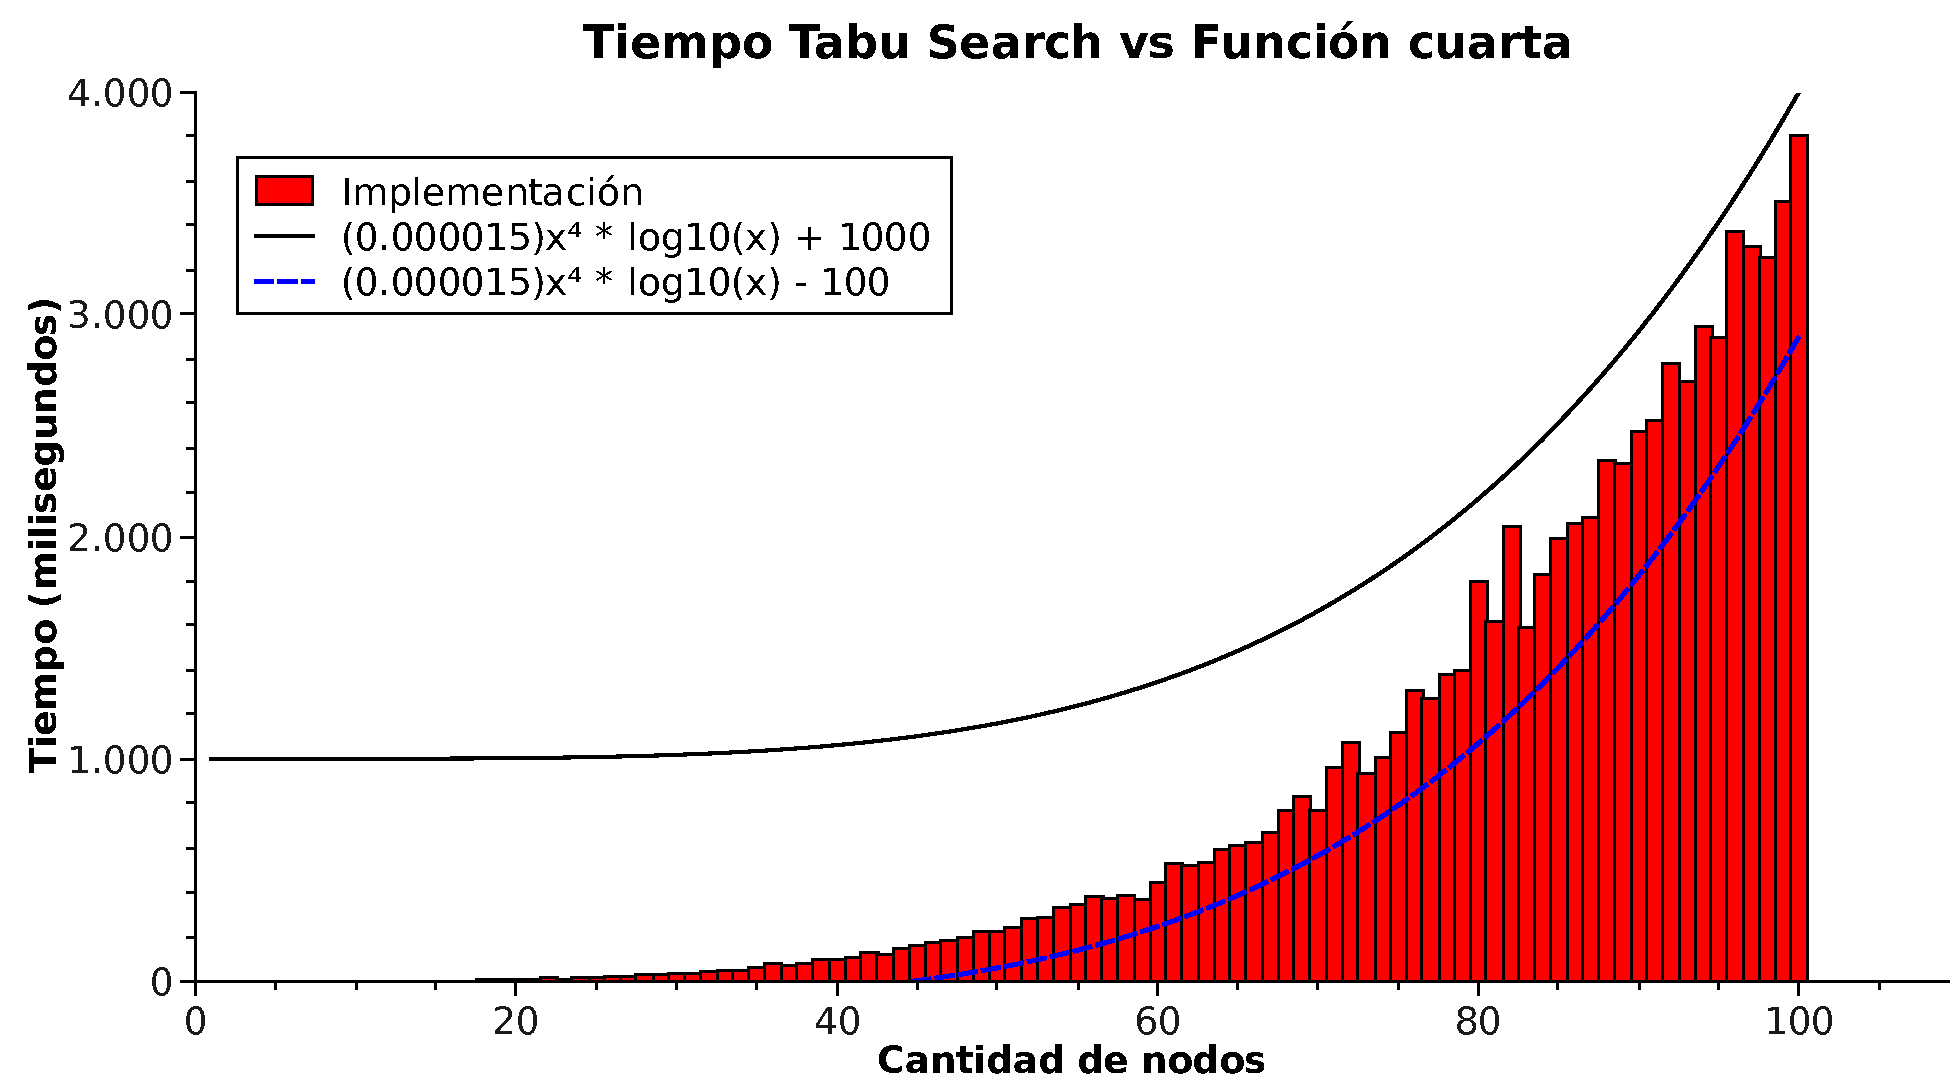
\includegraphics[width=\textwidth]{./otros/graficos/tiempo_100nodos1_ej5.pdf}
	\caption{}
	\label{ej5tiempo1}
\end{center}
\end{minipage}

% grafico 2
\begin{minipage}{\textwidth}
\begin{center}
	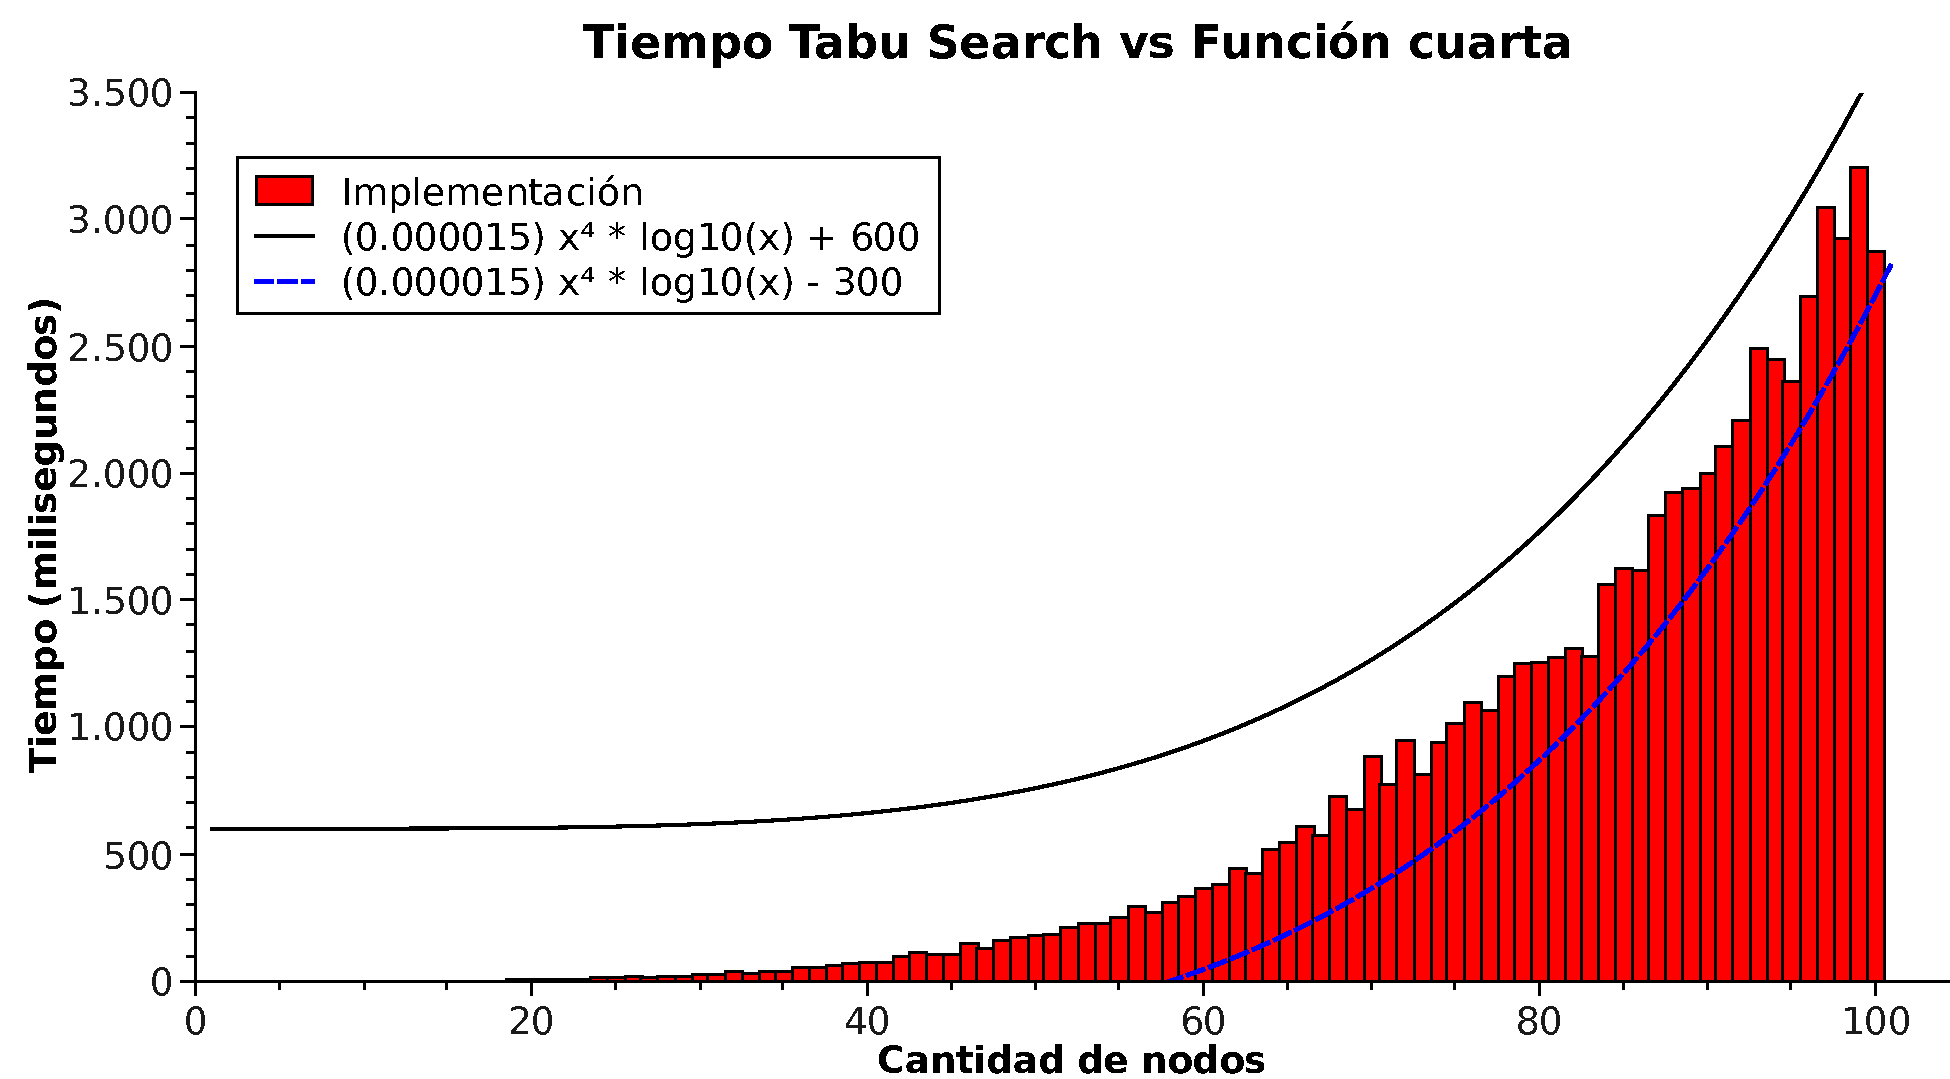
\includegraphics[width=\textwidth]{./otros/graficos/tiempo_100nodos2_ej5.pdf}
	\caption{}
	\label{ej5tiempo2}
\end{center}
\end{minipage}
\end{figure}

\begin{figure}[htb]
% grafico 3
\begin{minipage}{\textwidth}
\begin{center}
	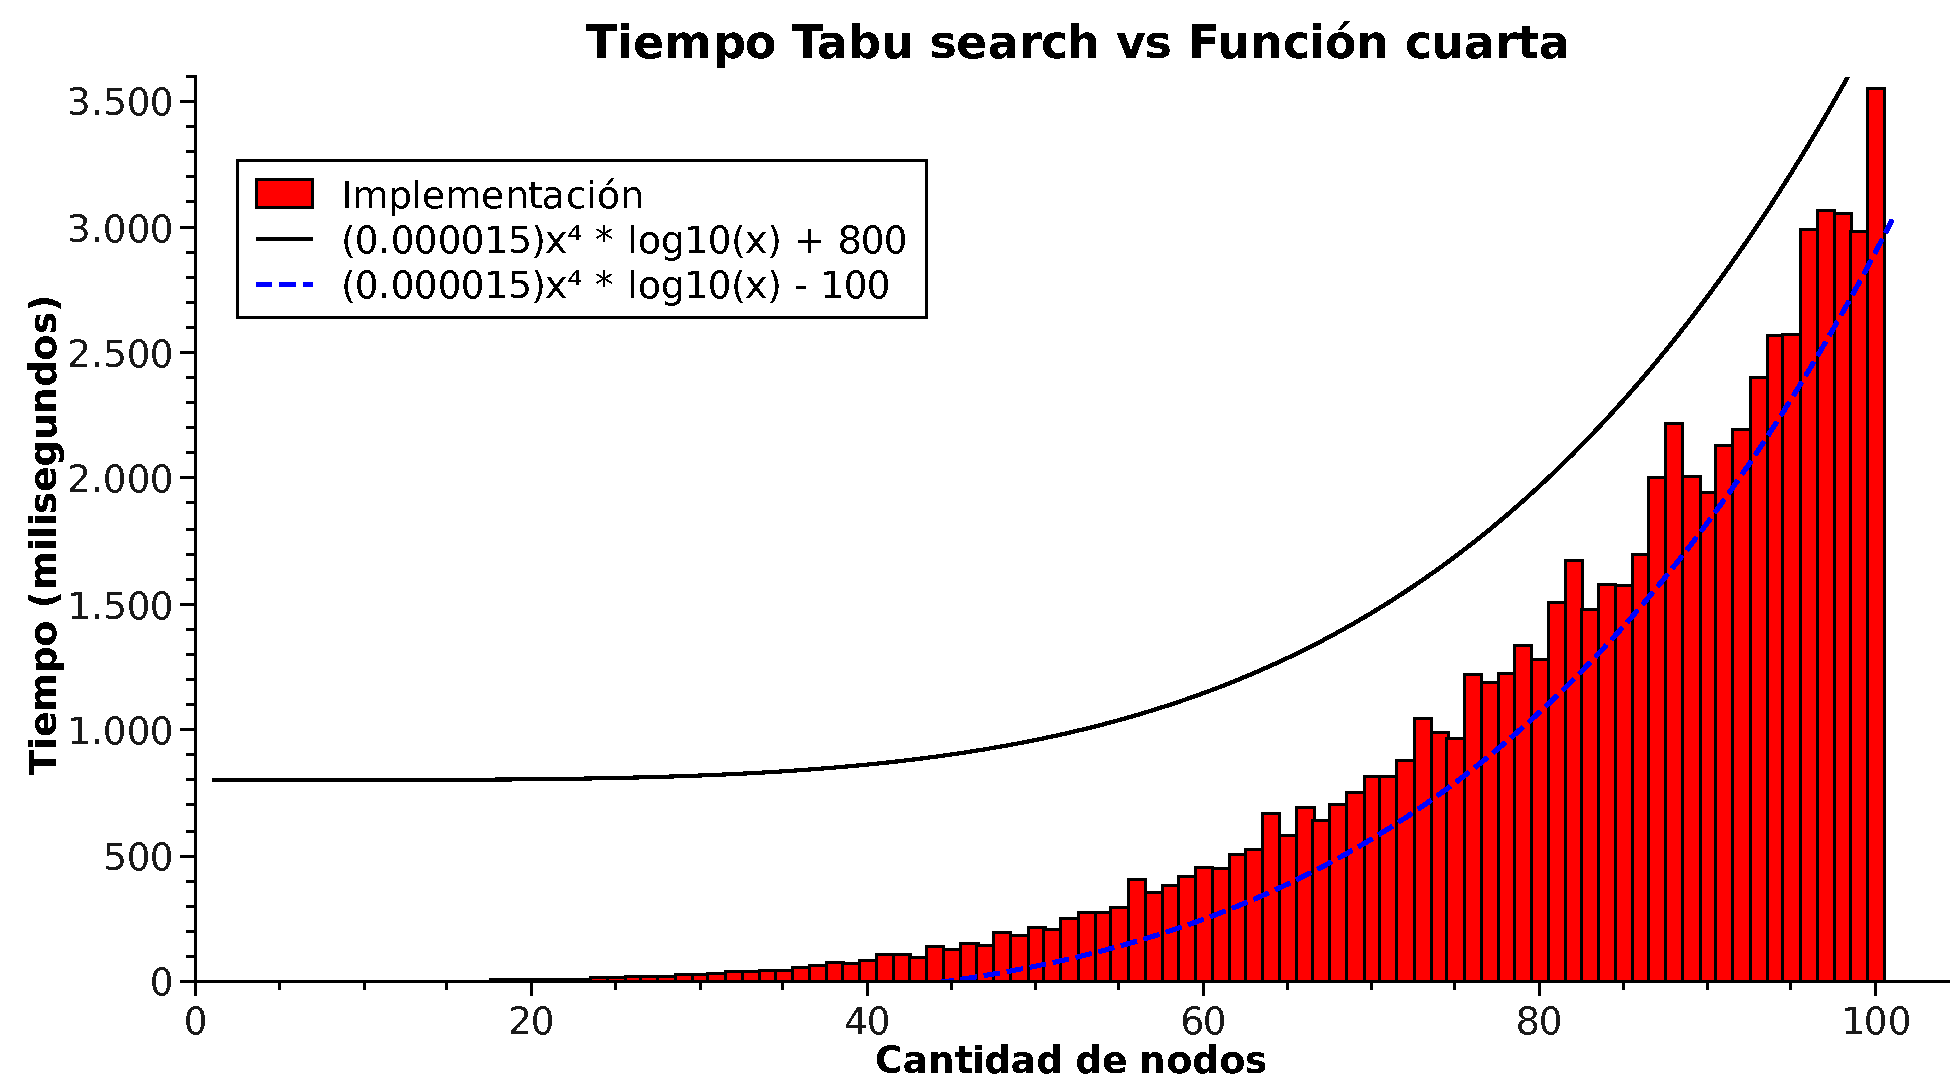
\includegraphics[width=\textwidth]{./otros/graficos/tiempo_100nodos3_ej5.pdf}
	\caption{}
	\label{ej5tiempo3}
\end{center}
\end{minipage}

% grafico 4
\begin{minipage}{\textwidth}
\begin{center}
	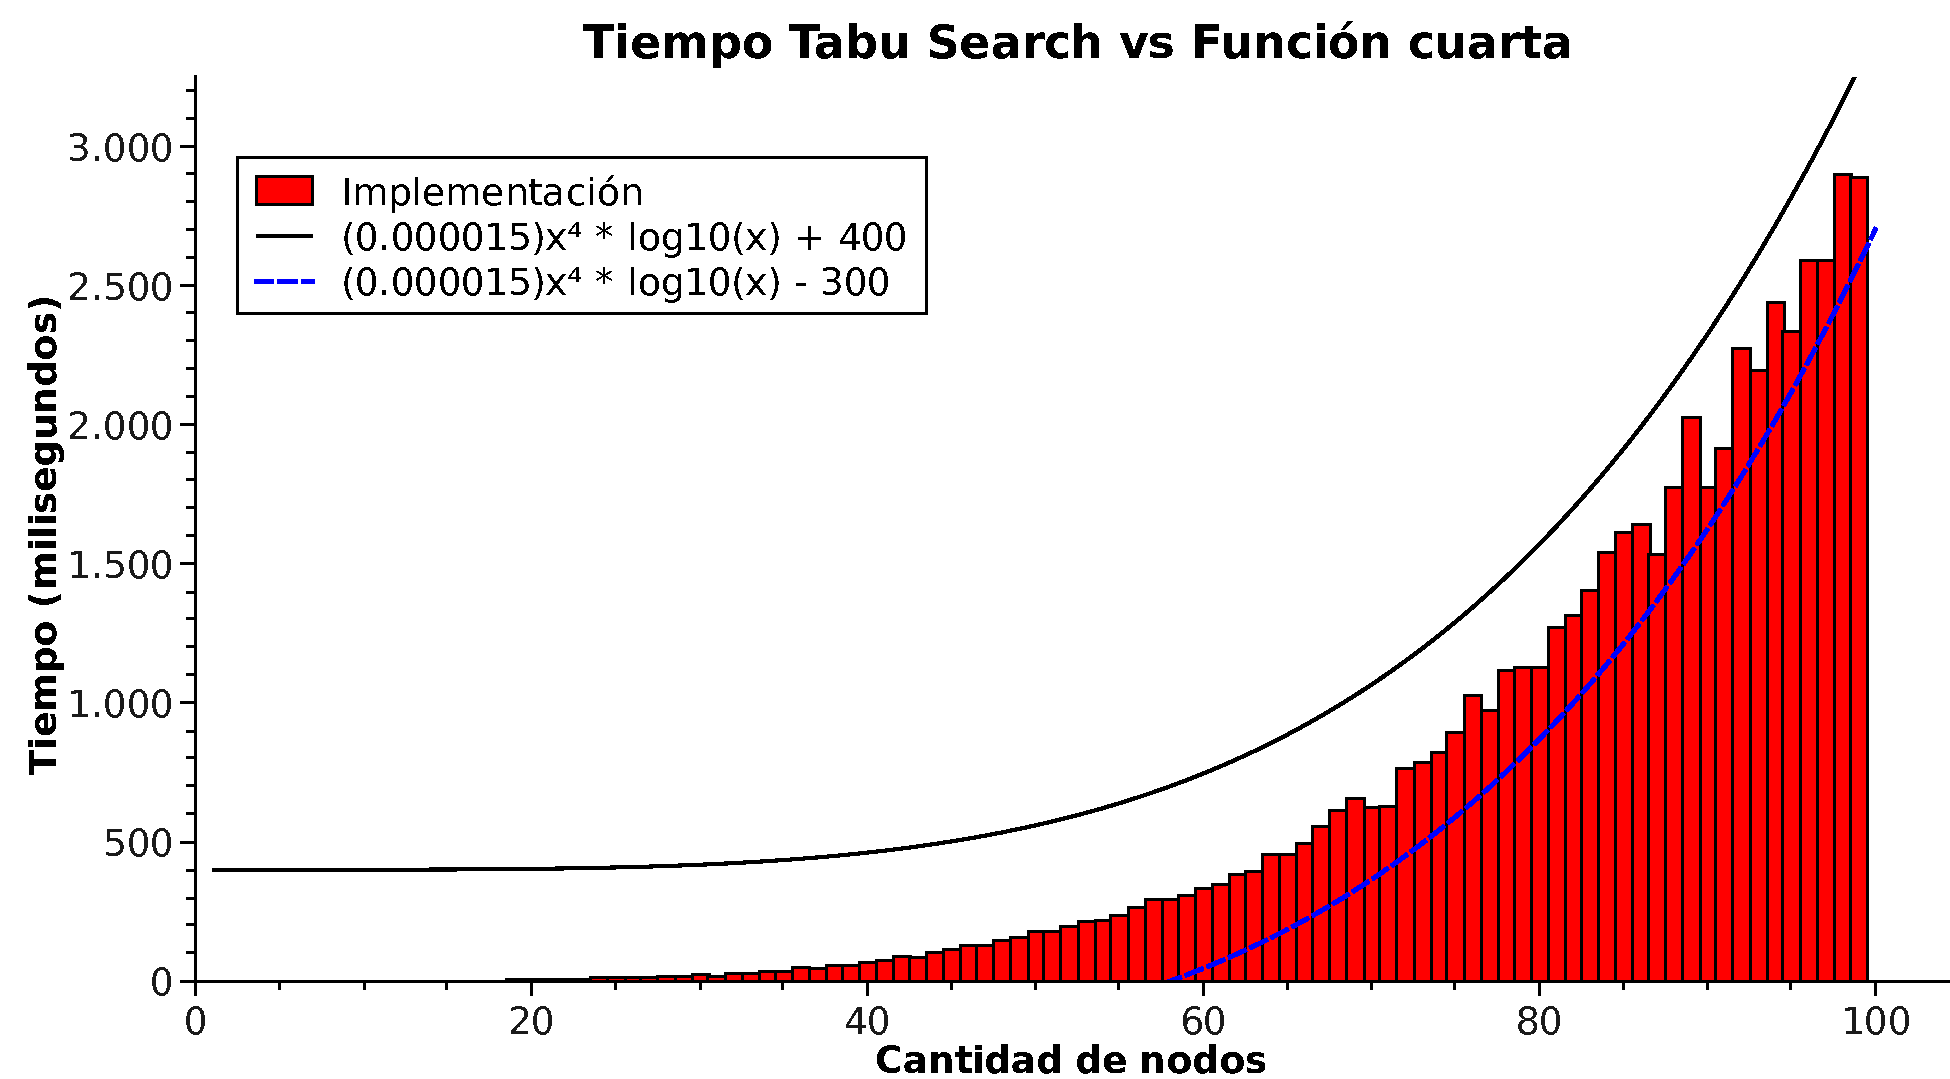
\includegraphics[width=\textwidth]{./otros/graficos/tiempo_100nodos4_ej5.pdf}
	\caption{}
	\label{ej5tiempo4}
\end{center}
\end{minipage}
\end{figure}

\subsection{Debate y Conclusiones}
\paragraph{}
El principal aspecto esperable del comportamiento de la metaheurística de búsqueda tabú es que requiera un mayor período de tiempo para resolver los mismos casos de prueba que las demás heurísitcas implementadas en este trabajo. Esto puede entenderse si se tiene en cuenta que si bien la metaheurística demora un tiempo significaticamente menor en relación el algoritmo exacto para obtener una solucion \footnote{Es lógico que así sea pues esa es básicamente la motivación para desarollar una heurística}, ésta si idea con el propósito de mejores que soluciones que las demás heuristicas mediante el uso de diversas técnicas y métodos de exploración del grafo. Por tanto cabe presuponer que 


%Una de las primeras cosas que se puede inferir de los gráficos presentados en la sección anterior es que en las pruebas realizadas la metaheurística se comportó de la manera prevista, ya que en todos ellos se pudo acotar los tiempos tanto inferior como superiormente por una función $f(x) = c.x^4 * log(x) + d$, con c y d contantes enteras. Según los datos arrojados por los gráficos en la sección anterior, podemos ver que los datos arrojados por las distintas corridas del algoritmo de búsqueda local tienen la forma que se esperaba. En la sección [\ref{complejidad4}], se explicó y analizó la complejidad de esta heurística, y se concluyó que la misma era \Ode{}. Dentro de estos gráficos, se ve que en estos casos de prueba, la heurística parece haberse comportado como era esperado, y pudo ser acotada por arriba y abajo por una función cuarta multiplicada por un logaritmo.Como se comentó en la sección de debate y conclusiones del ejercicio 3, a pesar de haberse tomado varias muestras en las que se variaba el número de ejes y de nodos, todos los resultados presentaban la misma forma, salvo alguna constante no muy pronunciada. Por ello no pareció adecuado incluir más gráficos, ya que en general y utilizando los generadores implementados por el grupo para este trabajo práctico, el comportamiento no varió de muestra en muestra.Podemos concluir entonces que el algoritmo, tanto en la teoría como en la práctica para los casos de prueba realizados se comportó como se esperaba, arrojando una complejidad de \Ode{n^4 * log(n)}.

